\documentclass[10pt, conference]{IEEEtran}

\newcommand{\ignore}[1]{}

% *** GRAPHICS RELATED PACKAGES ***
\usepackage[pdftex]{graphicx}
\usepackage{xcolor}
\usepackage{caption} %needed to make captions on figure* centered
\graphicspath{{./figures/}}
\DeclareGraphicsExtensions{.pdf,.png}
\usepackage[]{hyperref}

\usepackage[linesnumbered, ruled, vlined]{algorithm2e}

% correct bad hyphenation here
\hyphenation{Tele-operable}



% paper title
\title{STOIC: Serverless Teleoperable Hybrid Cloud for Machine Learning Applications on Edge Device}


\author{\IEEEauthorblockN{Michael Zhang, Chandra Krintz, Rich Wolski}
\IEEEauthorblockA{Dept. of Computer Science \\
University of California, Santa Barbara\\
\{lebo, ckrintz, rich, mock\}@cs.ucsb.edu}
}

%\author{\IEEEauthorblockN{Omitted for Blind Review}%\\
%\IEEEauthorblockA{Blind Review \\
%Blind Review\\
%&\{blind\}@blind.blind.blind}
%}

\begin{document}


% make the title area
\maketitle

\begin{abstract}
\label{sec:abstract}
Serverless computing emerges as a promising execution framework on the cloud for machine learning applications, considering the flexibility and elasticity it offers. However, the imbalance of computing resources between edge and public cloud dampens the availability and efficiency of serverless architecture, and consumes extraneous energy and costs from end users. 

The goal of our work is to bridge this gap by intelligently deploying tasks and making accelerator(e.g. GPU) serve edge devices in a robust and fault-tolerant fashion on serverless architecture. To enable this, we developed an open source cloud system called STOIC (Serverless TeleOperable HybrId Cloud), which leverages accelerators as a serverless service and schedules machine learning tasks across hybrid cloud system. Through our evaluation, STOIC largely outperforms single-runtime systems on real-world applications for IoT device and edge cloud. In this paper, we present the design and implementation of STOIC, along with the empirical evaluation of its efficacy and performance for machine learning applications.
\end{abstract}

\begin{IEEEkeywords}
Serverless computing; Model optimization; Hyperparameter tuning
\end{IEEEkeywords}


% For peer review papers, you can put extra information on the cover
% page as needed:
% \ifCLASSOPTIONpeerreview
% \begin{center} \bfseries EDICS Category: 3-BBND \end{center}
% \fi
%
% For peerreview papers, this IEEEtran command inserts a page break and
% creates the second title. It will be ignored for other modes.
\IEEEpeerreviewmaketitle



\section{Introduction}
\label{sec:intro}
Upon the recent shift of application architectures from monolithic to containers and microservices, serverless computing has risen as a promising cloud provider offering where event-driven functions compose all applications and services. It represents a revolutionary programming and deployment paradigm known as Function as a Service (FaaS). Using serverless model, developers can easily build up applications in a cloud without concerning server provisioning at the infrastructure level. Programmers usually write those functions in high-level languages and triggered by events either from external sources or, more often, internal cloud services. Thus, serverless architecture allows the application to distribute across the cloud by providing function-level abstraction.

Moreover, this function-level abstraction does not only abstract away the infrastructure management work from developers, but also, more importantly, provides more fine-grained computational resource isolation and usage, meaning each serverless function can autoscale independently based on the scale of incoming events. Providing such elasticity effectively avoids the single point failure and bottleneck service in a data-intensive application. From this perspective, serverless architecture is an ideal system for machine learning applications, especially for online training~\cite{ref:online} and model serving, because they usually transfer and handle a large amount of data, but the volume of each batch is uncertain and highly volatile depending on the data generated in that period. The flexibility that serverless functions deliver address such issue via the event-driven mechanism. 

To enable such an event-driven system, one concerning situation is that those machine learning applications usually evolve heterogeneous IoT devices, ranging from temperature sensors to mobile phones to autonomous drones, which are the primary data sources in the physical world. If the applications execute, at least partially, on the edge cloud, it could save lengthy round-trip time of transmitting data and make the application infinitely close to real-time. Such demand motivates us and we explore the effectiveness and efficiency of executing machine learning applications on the edge cloud in this work. 

An immediate difficulty we face is the scarcity of computational resources on edge cloud relative to high-demanding machine learning applications. In addition, no cloud provider offers serverless functions that leverage accelerators like GPU. In our work, we construct a hybrid cloud system that enables serverless function to utilize GPU, which substantially accelerates the execution of machine learning applications. We consider it as one of the key contributions of our research.

\begin{figure}
    \centering
    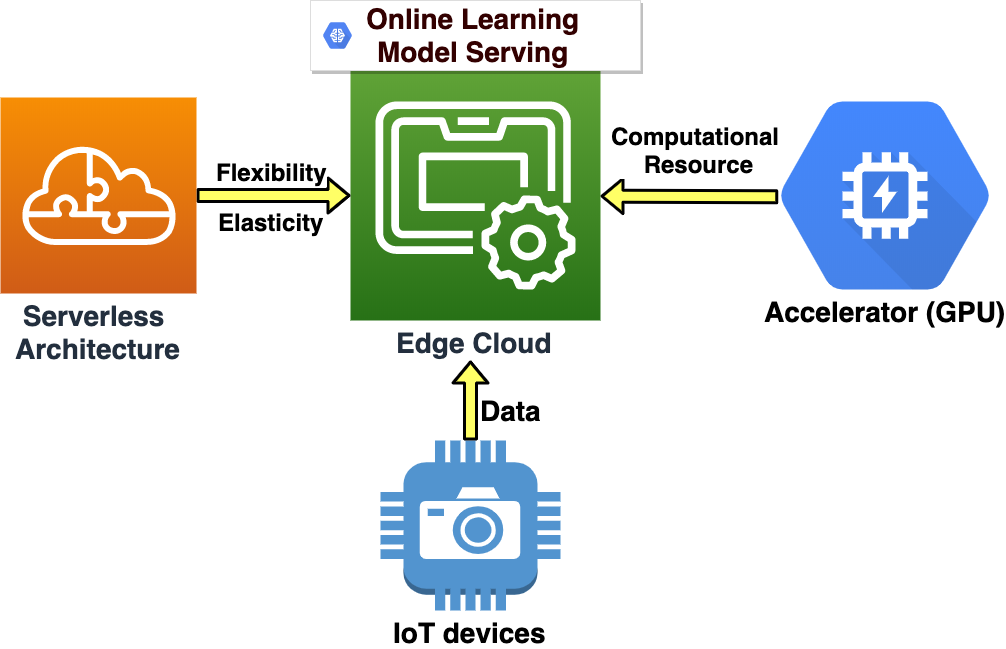
\includegraphics[scale=0.25]{figures/edge}
    \caption{\textbf{The Design Principle of STOIC}}
    \label{fig:edge}
\end{figure}

Figure~\ref{fig:edge} illustrates the design principles of our proposed system, STOIC (Serverless TeleOperable Hybrid Cloud). In our design, three underpinnings support the center edge cloud: IoT devices stream data in batches for training and inference; serverless architecture provides flexibility and elasticity to handle auto-scaling and unbalanced data payload; the accelerator offers an additional computational resource for extra large dataset and compute-intensive machine learning applications. In this paper, we discuss the design and implementation of this architecture, investigate the efficacy and  empirically evaluate its performance. We found STOIC reduces total response time, ranging from 6.48\% to 32.05\%, compared with four single runtimes. Finally, we show both related and future work and conclude.


%\section{Background}
%\label{sec:background}
%\input{background}

\section{STOIC}
\label{sec:STOIC}
To leverage accelerator and distributed scheduling using the serverless architecture, we have developed STOIC, a framework for executing machine learning applications in hybrid cloud consisting of edge devices and public data centers. The STOIC streamlines the end-to-end process of packaging, transferring, scheduling, executing and retrieving result for machine learning application. Figure~\ref{fig:STOIC} shows the architecture of STOIC, which is composed by three principle pillars: Edge cloud, Mayhem cloud and Nautilus cloud.

\begin{figure}[t] \centering 
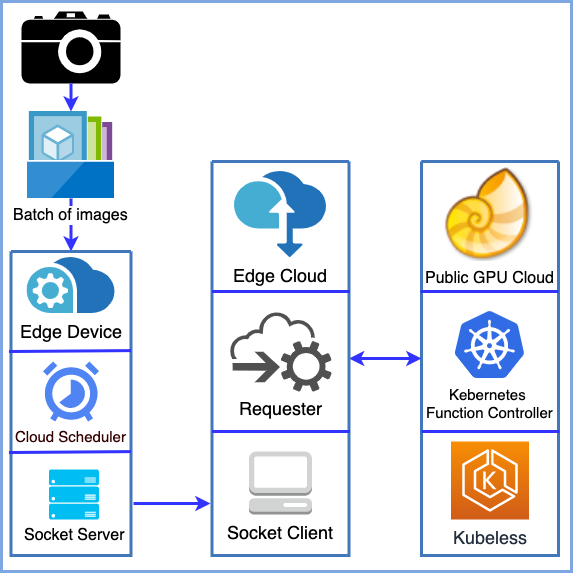
\includegraphics[scale=0.4]{STOIC}
\caption{The architecture of STOIC
\label{fig:STOIC}}
\end{figure}

\subsection{Edge Cloud}
 The edge cloud is a collection of edge devices, including multiple motion-detecting camera traps and local server, deployed in open field and research facility at Sedgwick Natural Reserve~\cite{ref:sedgwick}. Across the field, especially at the water pond, those camera traps are scattered to capture images of wildlife and are connected by microwave link networks to the local server in the research facility. When a motion is detected, the camera traps take photos and persist the images to the attached disk volume. Periodically, they transfer the photos to the local server in the facility, where STOIC socket server constantly listens for batch of images and STOIC cloud scheduler assigns the task to different cloud components. 
 
 \subsection{Mayhem Cloud}
 
 The Mayhem cloud is a private cloud built up by a cluster of nine Intel NUCs~\cite{ref:nucs}. It is managed by Eucalyptus cloud system~\cite{ref:euca} that supports Linux virtual machine instance of Ubuntu and CentOS. Running on an instance, the STOIC socket client listens for the request from edge cloud and STOIC requester interacts with Nautilus Cloud to complete the designated task.
 
 \subsection{Nautilus Cloud}
 
 The Nautilus Cloud~\cite{ref:nautilus} is a HyperCluster research platform led by researchers at UC San Diego, National Science Foundation, Department of Energy and various participating universities globally. Being designed for running data and computation intensive applications, Nautilus uses Kubernetes~\cite{ref:k8s} as interface to manage and scale containerized applications and Rook to automate Ceph~\cite{ref:ceph} data services. As of Nov. 2019, 141 computing nodes across the US joined Nautilus Cloud and 422 GPUs are available in the cluster. We consider Nautilus as an ideal public cloud to leverage accelerators in Serverless architecture to serve edge devices. 
 
 \subsection{Implementation}
 
 \subsubsection{Language}
 Considering performance and interface, STOIC is primarily developed in Golang, since the language provides better performance than scripting language like Python, as well as user-friendly interface~\cite{ref:client-go} to Kubernetes. 
 
 \BlankLine
 \subsubsection{Serverless framework}
 To enable Serverless architecture, STOIC employs kubeless~\cite{ref:kubeless} and Docker~\cite{ref:docker} at Nautilus Cloud. As a kubernetes-native serverless framewrok, kubeless uses CRD (Custom Resource Definition)\cite{ref:crd} to dynamically create functions as kubernetes custom resources and launches runtimes on-demand. For specific machine learning tasks that STOIC executes, we use Docker to build up customized runtime image and upload it to Docker Hub~\cite{ref:dockerhub}. Upon a task request is received, the function controller at Nautilus Cloud pulls the latest image from Docker Hub before launching the function. This deployment pipeline makes the runtime flexible and extensible for future modification. 
 
 \BlankLine
 \subsubsection{Customized Tensorflow}
 To better leverage the computational power of CPU in Edge and Nautilus Cloud, we compile a Tensorflow package from source with AVX2, SSE4.2~\cite{ref:avx} and FMA~\cite{ref:fma} instruction set support. We then test the performance of customized Tensorflow package on three common machine learning training tasks: \textbf{(A)} \textit{Iris}~\cite{ref:iris} with 10-fold cross-validation; \textbf{(B)} \textit{MNIST}~\cite{ref:mnist} on 20 Epochs; \textbf{(C)} \textit{InceptionV3}~\cite{ref:v3} on 10 epochs with 1,000 images. These applications are executed 10 times on both Tensorflow packages to ensure the result is reliable. Table~\ref{tab:avx} describes the performance comparison between two packages. Since the instruction set support accelerates the machine learning task on CPU runtime, we install the customized package to both Edge cloud and Nautilus Cloud Docker image to take advantage of the acceleration.
 
 \BlankLine
 \subsubsection{GPU Accessibility}
 To enable GPU access by Serverless function, we build up our runtime image based off NVIDIA Container Toolkit~\cite{ref:nvidia}. It includes NVIDIA runtime library and utilities to allow Serverless function to leverage NVIDIA GPUs. The resultant image is installed CUDA 10.0 and cuDNN 7.0, which are inline with most GPU nodes' version in Nautilus Cloud. 
 
\begin{table}[]
\centering
\scriptsize

\begin{tabular}{|c|c|c|c|} 
\hline
 & \textbf{Mean Std. (sec)} & \textbf{Mean Custom. (sec)} & \textbf{Speed-up \%}\\
\hline
\textbf{Iris} & 53.17 & 41.86 &  21.3\\
\hline
\textbf{MNIST} & 268.81 & 189.80 & 29.4 \\
\hline
\textbf{InceptionV3} & 958.47 & 791.28 & 17.4 \\
\hline
\end{tabular}

\caption{Performance comparison between standard and customized Tensorflow package}
\label{tab:avx}
\end{table}
 
 \BlankLine
 \subsubsection{Runtime definition}
 To effectively schedule the machine learning tasks, we define four runtime scenarios across hybrid cloud: \textbf{(A)} \textit{edge} - A VM instance at edge cloud on spot with AVX2 support; \textbf{(B)} \textit{cpu} - A pod with CPU with AVX2 support; \textbf{(C)} \textit{gpu1} - A pod with 1 GPU; \textbf{(D)} \textit{gpu2} - A pod with 2 GPUs. The last three runtimes are launched and invoked as kubeless functions at Nautilus Cloud. 
 
 For evaluation and canary release purpose, STOIC has a runtime flag implemented that overrides the runtime selection made by scheduler if the flag is set. This feature extensively helps evaluate the performance of STOIC comparing with single-runtime schedulers.
 
 
 \subsection{Execution Time Estimation}
 Depicted in Figure~\ref{fig:STOIC}, socket server in Edge Cloud keeps listening for images transmitted from camera traps. Upon the end of a preset period (currently 1 hour), STOIC predicts the total time of processing the present batch. The total time includes transfer time, runtime deployment time and corresponding processing time, based on 4 different runtime scenarios. 
 
 \subsubsection{Transfer time} It measures the time spent in transmitting compressed batch of images from Edge Cloud to Mayhem Cloud and Nautilus Cloud. It is calculated as ${T_{tran} = V_{bat} / B}$ where $V_{bat}$ represents the volume of batch and $B$ represents bandwidth at the time provided by a bandwidth monitor at Edge Cloud. 
 
 \subsubsection{Runtime deployment time} It measures the time Nautilus uses to deploy requested kubeless function. Since the scarcity of computation, it is obvious that \textit{gpu2} runtime takes longer to deploy than \textit{gpu1} and \textit{cpu} runtimes. We analyze the deployment log and calculate the average deployment time for each Nautilus runtime. In the future work, we plan to build up feedback control loop to dynamically update deployment time. Kindly notice that, for \textit{edge} runtime, the transfer and runtime deployment time zero out since the task is executed locally in the Edge Cloud.
 
 \subsubsection{Processing time} It is the execution time of specific machine learning task. As the primary component for scheduling task across hybrid cloud, we regress it based on prior experiment data by Bayesian Ridge Regression~\cite{ref:brr} due to its robustness to ill-posted problems compared to Ordinary Least Squares~\cite{ref:ols}. Thus, STOIC formulates the regression and predicts the processing time based on the size of current batch. As same as the deployment time, we plan to construct feedback control loop to dynamically update the coefficient and intercept of regression based on the incoming data of processing time in the future work.
 
 
 \subsection{Workflow}
 Based on three time components aforementioned, the execution times of four scenarios are predicted, and the scheduler selects the runtime with least time. If the choice is \textit{edge} runtime, scheduler will simply execute the task locally in the Edge Cloud. It usually happens when the batch of image is relatively small and does not require much computation from public cloud.
 
 However, when the batch size increases, the task is highly likely to be scheduled at three Nautilus runtimes. For these three scenarios, STOIC sends request, including the payload of compressed image batch and runtime information, to Mayhem Cloud via TCP socket. Upon reception of the request, Mayhem Cloud first requests the deployment of corresponding runtime and secondly sends the payload and request to Nautilus Cloud when the kubeless function is deployed. As a design decision, instead of running a serving pod in Nautilus, we decide to run a server in more stable and fault-tolerant Mayhem Cloud as a relay, due to the intermittent downtime on Nautilus nodes and Ceph storage system. This design provides more reliable infrastructure for tasks executing on STOIC.
 
 On the other end, Nautilus Cloud persists the received images to the shared storage in Ceph file system and monitors the progress of deployment of kubeless function. Once the the serverless function is successfully deployed, Nautilus informs the Mayhem Cloud whose requester will trigger the function via HTTP request. When the task completes, the requester retrieves the results, including the runtime metrics, and transmits them back to Edge Cloud, in which the results and metrics are saved. Up to this point, a full cycle of task execution on Serverless architecture has completed.
 
 \subsection{Intelligent Probing}
 In a series of experiment, we found the processing times of the same image batch and kubeless function vary significantly between first one and following ones. This is caused by cold start~\cite{ref:coldstart} problem of Serverless function. Specifically, most machine learning tasks require retrieval of stored model and dataset from shared file system, which might reside in a separate remote node in Nautilus Cloud. Once they are retrieved and cached in the first invocation, the function can simply use them from the local memory and the performance is boosted dramatically. To approach this issue, STOIC intelligently probes the recently deployed function based on the transition of runtime. When the incoming task is scheduled in a different runtime as previous one, STOIC triggers the function with least amount of data to ensure the model and data are cached in memory and then starts the actual task. Otherwise, to avoid redundant probing, STOIC starts the task directly when the designated runtime is the same as the previous batch. 

\section{Evaluation}
\label{sec:eval}
In this section, we empirically evaluate STOIC's performance on executing machine learning applications, in contrast to single-runtime systems. We first outline the machine learning application benchmark that we consider, followed by our test on the application efficacy. Then an empirical experiment and its result are presented.

\subsection{Benchmark Application and Dataset}

We benchmark STOIC using an image processing application that classifies animal images from a wildlife monitoring system called ``Where's The Bear" (WTB)~\cite{ref:wtb}. ``Where's The Bear" is an end-to-end distributed data acquisition and analytics system that implements an IoT architecture and edge cloud. Our application inferences streaming photos taken by wildly deployed camera traps in Sedgwick Natural Reserve using a convolutional neural network (CNN)~\cite{ref:cnn} model trained by labeled images from the WTB dataset. Technically, it employs Tensorflow and Scikit-learn~\cite{ref:scikit} machine learning frameworks to perform the image classification.  

 In total, there are five classes that we consider in the CNN model training: Bird, Fox, Rodent, Human and Empty. Since the volume of classes are unbalanced due to different occurring frequency of animals, we up-sample the minority classes (e.g. fox) by Keras ImageDataGenerator~\cite{ref:keras} to ensure the classification model is not biased. Every image in the WTB dataset is resized to $1920 \times 1080$, and for each class, the dataset contains 251 images used to train CNN model. Once the model is trained, the application caches this model in hdf5 format and store it at both edge cloud disk storage and a shared volume in Ceph file system at Nautilus cloud. 

\subsection{Application Efficacy}

\begin{table}[t] \centering 
\scriptsize
\resizebox{\columnwidth}{!}{
\begin{tabular}{|c|c|c|c|c|} 
\hline
& \textbf{Mean $T_r$ (sec)} & \textbf{Stdev. $T_r$ (sec)} & \textbf{Mean $T_p$ (sec)} & \textbf{Stdev. $T_p$ (sec)}\\
\hline
edge & 108.88 & 1.65 & 108.88 & 1.65 \\
\hline
cpu & 100.0 & 4.93 & 86.99 & 4.92 \\
\hline
gpu1 & 98.90 & 4.03 & 50.65 & 4.05 \\
\hline
gpu2 & 106.29 & 5.53 & 39.21 & 5.55\\
\hline
\textbf{STOIC} & \textbf{97.73} & \textbf{3.13} & \textbf{50.49} & \textbf{3.11} \\
\hline
\end{tabular}
}
\caption{\textbf{Mean and stdev of total response time~($T_r$) and processing time~($T_p$) of 40-image batch}: STOIC schedules tasks onto the runtime (\textit{gpu1}) that has the least total response time~($T_r$).
\label{tab:validation}}
\end{table}

We first test the efficacy of STOIC by processing an image batch of fixed size at four runtimes individually and then compare with STOIC. To make the result reliable, we again conduct the experiment 10 times and list the mean and standard deviation of total response time~($T_r$) and processing time~($T_p$) in Table~\ref{tab:validation}. We can observe from Table~\ref{tab:validation} that STOIC schedules 40-image batch to \textit{gpu1} runtime, based on its prediction that  \textit{gpu1} would have the least total response time~($T_r$). One important observation is that \textit{gpu2} runtime has even lower processing time~($T_p$) than \textit{gpu1}, but STOIC disregard \textit{gpu2} in this scenario, because its gain in processing time~($T_p$) does not compensate its lengthy deployment time~($T_d$) on Nautilus cloud.

\begin{figure}[t] \centering 
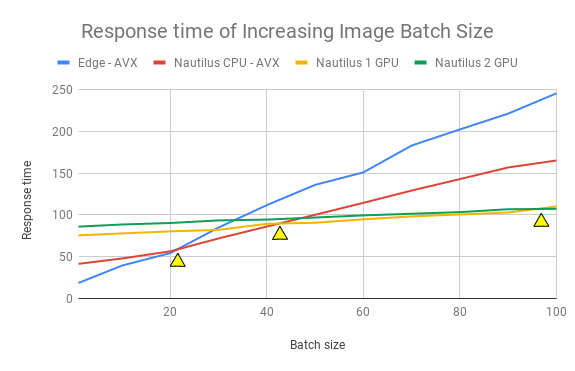
\includegraphics[scale=0.32]{response-time}
\caption{\textbf{Total Response Time~($T_r$) of image batches of growing sizes}: The x-axis represents batch size, while y-axis is the total response time~($T_r$). STOIC, which is depicted in blue dashed line, schedules the task on the runtime with the least total response time.  
\label{fig:response-time}}
\end{figure}

Additionally, we test STOIC by processing a series of image batches of growing sizes both on four runtimes and STOIC. The progressive response times are depicted in Figure~\ref{fig:response-time}. The x-axis is the size of image batch and the y-axis is the total response time~($T_r$) in seconds. The red curve represents the linearly increasing latency from \textit{edge} runtime, whereas the yellow one depicts that for \textit{cpu} runtime at Nautilus cloud. We observe that its slope is more moderate than \textit{edge} runtime since CPUs in nodes of Nautilus cloud are usually more powerful than edge cloud. The pink and green curve represent the \textit{gpu1} and \textit{gpu2} runtime respectively and they intersect at the batch size of 95, at which STOIC would switch the deployment of task from \textit{gpu1} to \textit{gpu2}. The blue dashed line depicts the total response time~($T_r$) of STOIC, which is able to schedule a series of tasks to the runtime with the least latency. According to such result, we ensure STOIC improves system performance by dynamic scheduling based on image batch size.


\subsection{Empirical Experiment}


% \begin{table}[t]
%     \centering
%     \scriptsize

\begin{tabular}{|c|c|c|c|c|c|} 
\hline
\textbf{Runtimes}& \textbf{edge} & \textbf{cpu} & \textbf{gpu1} & \textbf{gpu2} & \textbf{STOIC} \\
\hline
Avg. $T_r$ (sec) & 2842.58 & 2065.59 & 2173.98 & 2201.02 & 1931.64 \\
\hline
Speed-up (\%) & 32.05 & 6.48 & 11.15 & 12.24 & N/A \\
\hline
\end{tabular}

%     \caption{\textbf{Average total response time~($T_r$) and speed-up on 24-hour dataset}: Comparing with four single runtimes, STOIC achieves lowest average latency and speed-up ranging from 6.48\% to 32.05\%. }
%     \label{tab:24-batches}
% \end{table}


As an empirical evaluation of STOIC, we compare the total response time~($T_r$) of multiple image batches of varying sizes by four single runtimes and STOIC. To accelerate the repetitive experiment, we developed a simulator to generate image batches based on the frequency distribution of WTB dataset. According to 2016 WTB dataset, the size of image batch fits to normal distribution $\mathbf{N}(\mu = 42.75, \sigma^2 = 39.5)$. Thus, the simulator generates 24 image batches in the edge controller to emulate streaming data in one day from open field camera traps. To conduct unbiased evaluation, we seed the simulator to make these 24 image batches consistent across all runtimes and STOIC. 

\begin{figure}[t] \centering 
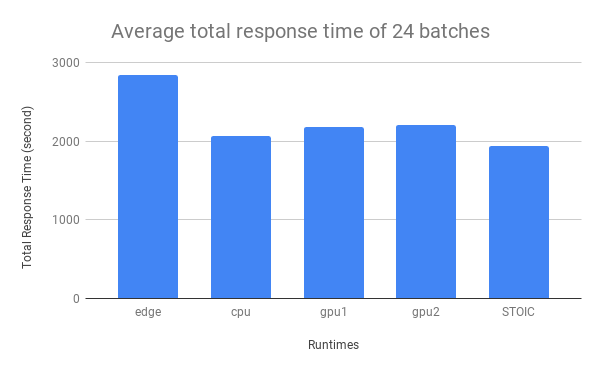
\includegraphics[scale=0.42]{figures/24-batches}
\caption{\textbf{Avg. total response time~($T_r$) on 24-hour dataset}: The x-axis represents runtimes, while y-axis represents the average total response time~($T_r$) by STOIC and four other runtimes on 24-hour dataset. The data labels on columns are specific numbers of $T_r$. The 24-hour batch sizes are generated from the distribution of historical data. 
\label{fig:24-batch}}
\end{figure}

To ensure the validity of outcome, We again run such experiment 10 times for each runtime scenario and report the average value. Figure~\ref{fig:24-batch} demonstrates the average total response time~($T_r$) for STOIC and four individual runtimes. Specifically, STOIC achieves the lowest average latency among four other single runtimes and reduces total response time~($T_r$) by 32.05\% (\textit{edge}), 6.48\% (\textit{cpu}), 11.15\% (\textit{gpu1}) and 12.24\% (\textit{gpu2}) respectively. According to such result, we conclude that STOIC outperforms single-runtime scheduling mechanism on empirical dataset and real-world machine learning application.


\section{Related Work}
\label{sec:relate_work}
As related work, we consider recent advances in both machine learning infrastructure and serverless computing domains. In the former area, much research has extended efforts into designing efficient systems for inference and deployment of machine learning models. As a complement to Tensorflow framework, Tensorflow-serving~\cite{ref:tensorflow-serving} integrates new models and updates versions from training to serving. Though it makes seminal exploration on the multi-tenant model hosting service, Tensorflow-serving does not realize authentic high-performing parallelism to handle concurrent heavy query loads. On that note, Clipper~\cite{ref:clipper} constructs a general-purpose low-latency prediction serving system, which attempts to solve the problem of demanding real-time prediction at the client-side and handling heavy query load at the server-side. It also enables the model composition and online learning to improve accuracy and render more reliable predictions. To explore the multi-pipeline techniques, PRETZEL~\cite{ref:pretzel} casts model-serving as a database problem and applies multi-query optimizations to maximize performance. However, both Clipper and PRETZEL could demand considerable compute resources in caching, batching, adaptive model selection and off-line training to maximize throughput. Therefore, they are not optimized for resource-constraint and heterogeneous IoT devices. To the best of our knowledge, STOIC is the first work to addresses this problem by integrating machine learning applications into a serverless architecture that leverages GPU as additional computational resources for IoT devices. We consider it as a promising and extensible solution for high-throughput and low-latency system for online training and machine learning applications in general. 

 To build up an end-to-end system for practical machine learning applications, we need several other components that bring it to fruition. Seneca~\cite{ref:seneca} fine-tunes hyper-parameters of machine learning models on a general-purpose serverless architecture, namely AWS Lambda~\cite{ref:lambda}. It provides a fast and low-cost method to grid search for the best-performing hyper-parameter set, which is essential in the deployment pipeline of machine learning applications. Velox~\cite{ref:velox} offers a low-latency and scalable solution for complex analytical model-serving, in which it completes a missing piece of personalized prediction serving using Apache Spark~\cite{ref:spark}. For calibrating the performance, McGrath et al.~\cite{ref:serverless} propose an empirical methodology to measure the design and performance of serverless platforms, including latency and auto-scaling capability. All these precursory work completes the serverless ecosystem, particularly for better training, inference and serving machine learning applications.


\section{Conclusion}
\label{sec:conclusion}
In this paper, we propose a framework, called STOIC, for executing machine learning applications in hybrid cloud settings based on serverless architecture. STOIC integrates three components: Edge Controller, Edge Cloud, and Public Cloud. When the scheduler at the edge controller receives a batch of images from open field camera traps, it predicts the total response time for processing the batch based on batch size and historical log data. It then schedules the task to the runtime that it predicts to have the least total response time.  Our STOIC prototype considers four different runtime scenarios. When STOIC schedules the task to the public cloud, the edge cloud deploys a serverless function and then relays the request and payload to the public cloud. STOIC returns the result and metrics to the edge controller when the task completes.

We present the design principles, implementation details, workflow and empirical evaluation on real-world machine learning application for STOIC. Our evaluation demonstrates STOIC is able to intelligently schedule machine learning tasks across hybrid cloud deployments and obtain better performance that using any single deployment option in isolation.  Our speed-up percentages range from 6.48\% to 32.05\% for the application and datasets that we study.

As part of future work, we are developing a feedback control loop to dynamically update the deployment and processing time of STOIC tasks. We plan to also investigate the feasibility of executing model-training tasks using STOIC. Finally, we plan to investigate ways of not having sufficient labeling for image classification tasks and to unify the serverless architecture across all edge and cloud systems within the STOIC system and for the applications that execute using it.



%\section*{Acknowledgments}
%This work is funded in part by NSF (CNS-1703560, OAC-1541215, CCF-1539586,
%CNS-1218808, ACI-1541215) ONR NEEC (N00174-16-C-0020), Huawei
%Corporation, and the California Energy Commission (PON-14-304).
%We also thank the  AWS Cloud Credits for Research program, which enabled us to
%perform this research.


% references section
\bibliographystyle{IEEEtran}
\bibliography{ref}
% \end{thebibliography}

\end{document}
